\documentclass[dvipdfmx,a4j]{jarticle}
\setlength{\textheight}{23.5cm}
\usepackage{tikz}
\usetikzlibrary{automata,calc,shapes}
\usepackage{tabularx}
\pagestyle{empty}
\newcounter{coffee}
\newcounter{bean}
\begin{document}
% \begin{flushright}
% \end{flushright}
\begin{center}
  {\bf\Large コンパイラ演習課題(2)(解答例)}
\end{center}


\begin{list}{\arabic{coffee}.}{\usecounter{coffee}}
  \item 逆ポーランド記法
        \begin{list}{(\alph{bean})}{\usecounter{bean}}
          \item \verb|a*b+c|\\
                \verb|ab*c+|
          \item \verb|a*b-c*(d+e)|\\
                \verb|ab*cde+*-|
        \end{list}
  \item
        \begin{list}{(\alph{bean})}{\usecounter{bean}}
          \item\ \\
                \[\left\{\begin{array}{rcl}
                    S  & \rightarrow & i E t S S',   \\
                    S  & \rightarrow & a         ,   \\
                    S' & \rightarrow & e S       ,   \\
                    S' & \rightarrow & \varepsilon , \\
                    E  & \rightarrow                 \\
                  \end{array}\right\}
                \]
          \item \ \\
                $i\;b\;t\;i\;b\;t\;a\;e\;a$に対して以下の２つの構文解析木が存在する．\\
                \begin{center}
                  \begin{tabularx}{.8\linewidth}{XX}
                    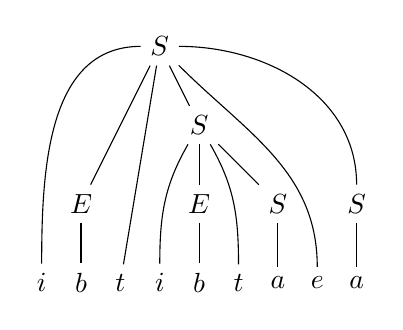
\begin{tikzpicture}
                      \node (Root) at (0,0) {$S$};
                      \node (N1) at (-1,-2) {$E$};
                      \node (N2) at (0.5,-1) {$S$};
                      \node (N3) at (0.5,-2) {$E$};
                      \node (N4) at (1.5,-2) {$S$};
                      \node (N5) at (2.5,-2) {$S$};
                      \node (N6) at (-1.5,-3) {$i$};
                      \node (N7) at (-1,-3) {$b$};
                      \node (N8) at (-0.5,-3) {$t$};
                      \node (N9) at (0,-3) {$i$};
                      \node (N10) at (0.5,-3) {$b$};
                      \node (N11) at (1,-3) {$t$};
                      \node (N12) at (1.5,-3) {$a$};
                      \node (N13) at (2,-3) {$e$};
                      \node (N14) at (2.5,-3) {$a$};
                      \path[-] (Root) [out=180,in=90] edge (N6);
                      \path[-] (Root) edge (N1) (Root) edge (N8) (Root) edge (N2);
                      \path[-] (Root) [out=315,in=90] edge (N13);
                      \path[-] (Root) [out=0,in=90] edge (N5);
                      \path[-] (N5) edge (N14);
                      \path[-] (N1) edge (N7) (N2) edge (N3) (N2) edge (N4);
                      \path[-] (N2) [out=240,in=90] edge (N9);
                      \path[-] (N3) edge (N10) (N4) edge (N12);
                      \path[-] (N2) [out=300,in=90] edge (N11);
                    \end{tikzpicture}
                     &
                    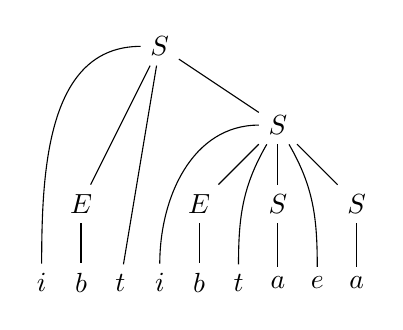
\begin{tikzpicture}
                      \node (Root) at (0,0) {$S$};
                      \node (N1) at (-1,-2) {$E$};
                      \node (N2) at (1.5,-1) {$S$};
                      \node (N3) at (0.5,-2) {$E$};
                      \node (N4) at (1.5,-2) {$S$};
                      \node (N5) at (2.5,-2) {$S$};
                      \node (N6) at (-1.5,-3) {$i$};
                      \node (N7) at (-1,-3) {$b$};
                      \node (N8) at (-0.5,-3) {$t$};
                      \node (N9) at (0,-3) {$i$};
                      \node (N10) at (0.5,-3) {$b$};
                      \node (N11) at (1,-3) {$t$};
                      \node (N12) at (1.5,-3) {$a$};
                      \node (N13) at (2,-3) {$e$};
                      \node (N14) at (2.5,-3) {$a$};
                      \path[-] (Root) [out=180,in=90] edge (N6);
                      \path[-] (Root) edge (N1) (N1) edge (N7) (Root) edge (N8);
                      \path[-] (Root) edge (N2);
                      \path[-] (N2) [out=180,in=90] edge (N9);
                      \path[-] (N2) edge (N3) (N3) edge (N10) (N2) edge (N4)
                      (N2) edge (N5) (N4) edge (N12) (N5) edge (N14);
                      \path[-] (N2) [out=240,in=90] edge (N11);
                      \path[-] (N2) [out=300,in=90] edge (N13);
                    \end{tikzpicture}
                  \end{tabularx}
                \end{center}
          \item\ \\
                \begin{tabular}{cc}
                  $G_1$                                         & $G'_1$ \\
                  \begin{tabular}{l}
                    {\bf 生成規則:}                                \\
                    $\begin{array}{cl}
                         1: & S \rightarrow\ i\, E\, t\, S         \\
                         2: & S \rightarrow\ i\, E\, t\, S\, e\, S \\
                         3: & S \rightarrow\ a                     \\
                         4: & E \rightarrow\ b                     \\
                       \end{array}$ \\[10pt]
                    {\bf LL(1) 構文解析表:}                         \\
                    \begin{tabular}{c|cccccc}
                          & $i$   & $t$ & $e$ & $a$ & $b$ & $\sharp$ \\ \hline
                      $S$ & 1 / 2 &     &     & 3   &     &          \\
                      $E$ &       &     &     &     & 4   &
                    \end{tabular}
                  \end{tabular} &
                  \begin{tabular}{l}
                    {\bf 生成規則:}                             \\
                    $\begin{array}{rcl}
                         1: & S \rightarrow   & i\,E\,t\,S\,S_1 \\
                         2: & S \rightarrow   & a               \\
                         3: & S_1 \rightarrow & e\,S            \\
                         4: & S_1 \rightarrow & \varepsilon     \\
                         5: & E \rightarrow   & b
                       \end{array}$ \\[10pt]
                    {\bf LL(1) 構文解析表:}                      \\
                    \begin{tabular}{c|cccccc}
                            & $i$ & $t$ & $e$   & $a$ & $b$ & $\$$ \\ \hline
                      $S$   & 1   &     &       & 2   &     &      \\
                      $S_1$ &     &     & 3 / 4 &     &     & 4    \\
                      $E$   &     &     &       &     & 5   &
                    \end{tabular}
                  \end{tabular}
                \end{tabular}
        \end{list}
  \item\ \\
        \begin{list}{(\alph{bean})}{\usecounter{bean}}
          \item \begin{eqnarray*}
                  \textsf{First}(\varepsilon) &=& \{\varepsilon\} \\
                  \textsf{First}(B) &=& \{w\} \\
                  \textsf{First}(D) &=& \{\varepsilon, x, y\} \\
                  \textsf{First}(E) &=& \{\varepsilon, y\} \\
                  \textsf{First}(F) &=& \{\varepsilon, x\} \\
                  \textsf{First}(S) &=& \{u\} \\
                  \textsf{First}(v) &=& \{v\} \\
                  \textsf{First}(w) &=& \{w\} \\
                  \textsf{First}(x) &=& \{x\} \\
                  \textsf{First}(y) &=& \{y\} \\
                  \textsf{First}(z) &=& \{z\} \\
                  \textsf{First}(B\,v) &=& \{w\} \\
                  \textsf{First}(D\,z) &=& \{x, y, z\} \\
                  \textsf{First}(E\,F) &=& \{\varepsilon, x, y\} \\
                  \textsf{First}(B\,D\,z) &=& \{w\} \\
                  \textsf{First}(u\,B\,D\,z) &=& \{u\}
                \end{eqnarray*}
          \item \begin{eqnarray*}
                  \textsf{Follow}(S) &=& \{\#\} \\
                  \textsf{Follow}(B) &=& \{v,x,y,z\} \\
                  \textsf{Follow}(D) &=& \{z\} \\
                  \textsf{Follow}(E) &=& \{x,z\} \\
                  \textsf{Follow}(F) &=& \{z\}
                \end{eqnarray*}
          \item 生成規則に番号をふる．\\
                $\begin{array}{rcl}
                    1: & S & \rightarrow u\,B\,D\,z  \\
                    2: & B & \rightarrow B\,v        \\
                    3: & B & \rightarrow w           \\
                    4: & D & \rightarrow E\,F        \\
                    5: & E & \rightarrow y           \\
                    6: & E & \rightarrow \varepsilon \\
                    7: & F & \rightarrow x           \\
                    8: & F & \rightarrow \varepsilon
                  \end{array}$
                下向き構文解析表：
                \begin{tabular}{c|ccccccc}
                      & $u$ & $v$ & $w$   & $x$ & $y$ & $z$ & $\$$ \\ \hline
                  $S$ & 1   &     &       &     &     &     &      \\
                  $B$ &     &     & 2 / 3 &     &     &     &      \\
                  $D$ &     &     &       & 4   & 4   & 4   &      \\
                  $E$ &     &     &       & 6   & 5   & 6   &      \\
                  $F$ &     &     &       & 7   &     & 8   &
                \end{tabular}

                $(B,w)$に適用ルールの競合があるので，LL1ではない．
          \item $B_{tail}$を新たに導入する．
                \[P_2=\left\{\begin{array}{ll}
                    1: S\rightarrow uBDz ,                 & 6: E\rightarrow y          , \\
                    2: B\rightarrow w B_{tail}   ,         & 7: E\rightarrow\varepsilon , \\
                    3: B_{tail}\rightarrow v B_{tail}    , & 8: F\rightarrow x          , \\
                    4: B_{tail}\rightarrow \varepsilon,    &                              \\
                    5: D\rightarrow EF   ,                 & 9: F\rightarrow\varepsilon
                  \end{array}\right\}\]

                \begin{tabular}{c|ccccccc}
                                      & $u$ & $v$ & $w$ & $x$ & $y$ & $z$ & $\$$ \\ \hline
                  $S$                 & 1   &     &     &     &     &     &      \\
                  $B$                 &     &     & 2   &     &     &     &      \\
                  $B_{\mathrm{tail}}$ &     & 3   &     & 4   & 4   & 4   &      \\
                  $D$                 &     &     &     & 5   & 5   & 5   &      \\
                  $E$                 &     &     &     & 7   & 6   & 7   &      \\
                  $F$                 &     &     &     & 8   &     & 9   &
                \end{tabular}
          \item \begin{eqnarray*}
                  S & \Rightarrow_{1} & u\,B\,D\,z \\
                  & \Rightarrow_{2} & u\,w\,B_{\mathrm{tail}}\,D\,z \\
                  & \Rightarrow_{3} & u\,w\,v\,B_{\mathrm{tail}}\,D\,z \\
                  & \Rightarrow_{3} & u\,w\,v\,v\,B_{\mathrm{tail}}\,D\,z \\
                  & \Rightarrow_{4} & u\,w\,v\,v\,D\,z \\
                  & \Rightarrow_{5} & u\,w\,v\,v\,E\,F\,z \\
                  & \Rightarrow_{6} & u\,w\,v\,v\,y\,F\,z \\
                  & \Rightarrow_{8} & u\,w\,v\,v\,y\,x\,z
                \end{eqnarray*}

                \begin{tikzpicture}[
                    level distance=12mm,
                    level 1/.style={sibling distance=30mm},
                    level 2/.style={sibling distance=17mm},
                    level 3/.style={sibling distance=14mm},
                    level 4/.style={sibling distance=12mm},
                    every node/.style={inner sep=2pt},
                    edge from parent/.style={draw}
                  ]
                  \node {$S$}
                  child {node {$u$}}
                  child {node {$B$}
                      child {node {$w$}}
                      child {node {$B_{\mathrm{tail}}$}
                          child {node {$v$}}
                          child {node {$B_{\mathrm{tail}}$}
                              child {node {$v$}}
                              child {node {$B_{\mathrm{tail}}$}
                                  child {node {$\varepsilon$}}
                                }
                            }
                        }
                    }
                  child {node {$D$}
                      child {node {$E$}
                          child {node {$y$}}
                        }
                      child {node {$F$}
                          child {node {$x$}}
                        }
                    }
                  child {node {$z$}};
                \end{tikzpicture}
        \end{list}
\end{list}
\end{document}
